
%(BEGIN_QUESTION)
% Copyright 2011, Tony R. Kuphaldt, released under the Creative Commons Attribution License (v 1.0)
% This means you may do almost anything with this work of mine, so long as you give me proper credit

Examine the P\&ID for this crude oil heater -- one of the first stages of crude oil distillation where the oil is split up into its constituent components -- then answer the following questions:

$$\includegraphics[width=15.5cm]{i02503x01.eps}$$

\begin{itemize}
\item{} Explain how this control system is supposed to function, with two transmitters, two controllers, and only one control valve.
\vskip 10pt
\item{} Identify the proper action of the FIC ({\it direct} or {\it reverse}).
\vskip 10pt
\item{} The low-limit function block (FY) located between the FIC and the flow-control valve is supposed to function as a {\it minimum flow} override to the FIC.  Explain the purpose in having such an override in this heater control system.
\vskip 10pt
\item{} How will the control system react to an operator opening up the fuel gas valve further?
\vskip 10pt
\item{} Identify at least one fault that could cause the flow control valve to shut fully despite the action of the low-limit relay.
\end{itemize}


\vskip 20pt \vbox{\hrule \hbox{\strut \vrule{} {\bf Suggestions for Socratic discussion} \vrule} \hrule}

\begin{itemize}
\item{} A useful analytical technique for any complex control system is to annotate the diagram with ``+'' and ``$-$'' symbols at the instrument bubble inputs, designating ``noninverting'' and ``inverting'' characteristics, respectively.  Show how this helps you track of all directions of action, making it easier to figure out how the control system responds to changes.
\item{} Could the low-limit function be relocated to a place between the two controllers, so as to limit the cascaded setpoint signal to some minimum value and thereby achieve the same effect?  Explain why or why not.
\end{itemize}

\underbar{file i02503}
%(END_QUESTION)





%(BEGIN_ANSWER)


%(END_ANSWER)





%(BEGIN_NOTES)

This is a cascade control system, where a temperature controller provides a setpoint to a feed flow controller to maintain stable outlet temperature from the heater.

\vskip 10pt

The FIC needs to be reverse-acting to control flow through the heater.

\vskip 10pt

The low-limit function block provides a minimum flow override to the flow controller, preventing it from closing the control valve any further than 10\% open.  This is to prevent tube overheating due to insufficient oil flow through them.

\vskip 10pt

As the fuel valve is opened further, outlet temperature will rise, prompting the TIC to call for more flow from the FIC.  The feed flow valve opens up, allowing more cool oil to enter the heater and thus reduce the outlet temperature.

\vskip 10pt

Any fault in the I/P causing low output pressure (e.g. plugged supply line, plugged restrictor) would cause the control valve to fail shut despite the 10\% low limit function block.

$$\includegraphics[width=15.5cm]{i02503x02.eps}$$

\vfil \eject

\noindent
{\bf Prep Quiz:}

Identify the purpose of the low-limit function (FY) in this control system:

$$\includegraphics[width=15.5cm]{i02503x01.eps}$$

\begin{itemize}
\item{} Prevents the control valve from completely shutting
\vskip 5pt 
\item{} Limits the maximum temperature of the heated product
\vskip 5pt 
\item{} Prevents the controller's integral action from "winding" up
\vskip 5pt 
\item{} Limits the rate-of-change of temperature in the heater
\vskip 5pt 
\item{} Limits the setpoint value sent to the slave (flow) controller
\vskip 5pt 
\item{} Prevents the control valve from completely opening
\end{itemize}



%INDEX% Process: crude oil heater (fired)
%INDEX% Relay, computational: limit functions

%(END_NOTES)


